\documentclass[a4paper, 12pt]{article}

%\usepackage{savetrees}
\usepackage{graphicx}
\usepackage{subfig}
\usepackage{longtable}

%code for creating python code snippets
\usepackage{float}
\floatstyle{ruled}
\newfloat{python}{thp}{lop}
\floatname{python}{Listing}
%end code for creating python code snippets

\graphicspath{{./images/}}
\title {Student Robotics 2009\\ Assembly Guide}
\date{\today}
\setcounter{tocdepth}{1}


\begin{document}


\maketitle

\noindent This document explains how to connect up the Student Robotics electronics kit. It is a \textit{Getting Started Guide} and is not a comprehensive description of the hardware. For more information about individual boards, see the respective documentation, available from the website: http://www.srobo.org 

\section{Before You Begin}

Whilst some of the connecting cables are supplied to you, others will have to be put together yourself. Here is some general advice to follow when preparing your electronics kit:
\begin{itemize}
\item When assembling connectors you \textbf{must} follow the wiring guidelines as specified in the competition rules. This means using black wire for GND connections and red for 5V \& 12V. 
\item Keep wiring neat and securely terminated. Do not leave bare wires exposed. Keep connectors as short as possible.
\item \textbf{Never} make changes to your kit whilst it is switched on.
\item Mount \textbf{all} components securely using cable ties and the pcb standoffs supplied.

\end{itemize}


\section{Identify Kit Components}
Use the glossary in Section \ref{sec:glossary} to identify the different components. This will make the following stages easier.
\subsection{Types of Connector}
There are two types of connector used within the SR kit: 
\begin{itemize}
\item \textbf{RJ11 cables} - provide data connections (and small amount of power) to each of the boards, similar to USB cables. 
\item \textbf{SR Connectors} - supply power to some of the boards, the USB Hub and the battery.
\end{itemize} 


\section{Assembling the Power Board}
The power board is at the heart of the electronics kit and for this reason should be assembled first. You will need a copy of the \textbf{Power Board Outline} for this section.

\subsection{Switches}
\begin{enumerate}
\item Connect the \textbf{Charge/Run Switch} to the Power Board. 
\item Connect the \textbf{On/Off Switch} to the Power Board - be careful to locate the correct socket. Leave the switch in the `Off' position.
\end{enumerate}

\subsection{Power USB Hub}
\begin{enumerate}
\item Use the \textbf{USB Hub Power Connector} to connect the Hub to the Power Board
\item Use the \textbf{USB Cable} to connect the Hub to the `Disk 2' USB socket on the Slug - see Figure \ref{fig:slug-side}
\item Insert both \textbf{USB Keys} into sockets on the USB Hub
\end{enumerate}

\begin{figure}[h!]
\center
\includegraphics[scale=0.6]{slug-side-view}
\caption{Side view of the Slug's USB Ports}
\label{fig:slug-side}
\end{figure}


\subsection{The Slug}
Identify the Slug's Pin Header on the Power Board and \textbf{carefully} plug the Slug's multicoloured ribbon cable into it. Be sure to orientate the socket correctly, before applying force. This cable provides both power and data connections between the slug and, indirectly, all the SR modules.

\subsection{The Webcam}
Plug the \textbf{USB Webcam} into one of the spare USB sockets on the USB Hub.

\subsection{Fuse}
Your Power Board should have been supplied with a fuse already fitted. If yours hasn't, then contact a SR member as soon as possible.

\subsection{Battery \& Charger}
Connect the {\bf battery} to the {\bf Battery Connector} and plug the other end into the correct socket on the Power Board. {\bf Check the polarity carefully!}

Initially the battery will be uncharged, so plug the {\bf Battery Charger} into the socket on the Power Board and turn it on at the mains.


\subsection{Stop}
At this point you have assembled the minimum amount of kit to power up your robot. Ensure the Charge/Run Switch is in charge mode (see Power Board Documentation) and put the On/Off switch into the On position. If you have made no mistakes so far, the LEDs on the Power Board will be lit, the Slug will be flashing, and the lights on the USB hub and keys will also flash.

You may, at this point, write some python code to control the Power Board LEDs to satisfy yourself that everything is working.



\section{Assembling the Motor Board}
We will now connect the Motor Board to the rest of the kit. Ensure that you have {\bf turned your robot OFF before continuing}

\subsection{RJ11 Cable}
Use one of your RJ11 cables to connect the Power Board (you may use any one of the four RJ11 sockets) to the Motor Board.

\subsection{Motor Power}
Use the wire and SR Connectors to connect the Motor power supply on the Power Board to the socket on the Motor Board. Ensure that the +12V signal at the Power Board is connected to +12V signal at the Motor Board, and also that GND connects to GND. {\bf You will need to refer to the Motor and Power Board Outlines!}

\subsection{Motors}
Now use more wire and SR Connectors to connect your robot's motors to the Motor Board. You will need to refer to the Motor Board Documentation.

\subsection{Testing}
At this point you can write a simple python script to test that the motors are correctly installed. See the Programming Reference for more information


 



\newpage
\section{Assembling the PWM board}
The PWM Board, sometimes referred to as the Servo Board, controls up to 6 Servos and also features an LCD display which can be used during testing. Ensure that you have {\bf turned your robot OFF before continuing}

\subsection{RJ11 Cable}
Use one of your RJ11 cables to connect the Power Board (you may use any one of the four RJ11 sockets) to the PWM Board.

\subsection{Servo Power}
Use the wire and SR Connectors to connect the Servo power supply on the Power Board to the socket on the PWM Board. Ensure that the +5V signal at the Power Board end is connected to +5V signal at the PWM Board end, and also that GND connects to GND. {\bf You will need to refer to the PWM and Power Board Outlines!}

\subsection{Servos}
Refer to the PWM Board Documentation in order to connect your robot's servos to this board.

\subsection{Testing}
At this point you can write a simple python script to test that the servos and LCD are correctly installed. See the Programming Reference for more information.


 



\newpage
\section{Assembling the JointIO board}
The JointIO board provides analogue and digital Input/Output capabilities to your robot. Ensure that you have {\bf turned your robot OFF before continuing}

\subsection{RJ11 Cable}
Use one of your RJ11 cables to connect the Power Board (you may use any one of the four RJ11 sockets) to the JointIO Board.

The JointIO Board draws its power from the RJ11 connection, therefore it does not need an additional power supply.

\subsection{IO Devices}
Refer to the JointIO Board Documentation in order to connect your robot's IO devices to this board.

\subsection{Testing}
At this point you can write a simple python script to echo the value of its inputs at its outputs or to flash its outputs in a simple sequence. This will test that the board has been correctly installed. See the Programming Reference for more information.


 



\section{Conclusion}
Once you have tested each of the boards individually, you should write another python script to test all of the boards together. This will include testing the webcam. It is a very good idea to keep a copy of all of your test routines for use in the future when you make changes which inadvertently stop your robot working.

\newpage
%Glossary of components, terms

\section{Glossary}
\label{sec:glossary}
\begin{longtable}{| l | l| l |}
\hline
\textbf{Component} & \textbf{Description} & \textbf{Quantity} \\ \hline
\includegraphics[width=4cm]{chrg-run-sw}  & Charge/Run switch & 1 \\ \hline
\includegraphics[width=4cm]{on-off-sw}  & On/Off Switch & 1 \\ \hline
\includegraphics[width=4cm]{battery-con}  & Battery Connector & 1 \\ \hline
\includegraphics[width=4cm]{wire}  & Multi-core Electrical Wire & 5 \\ \hline
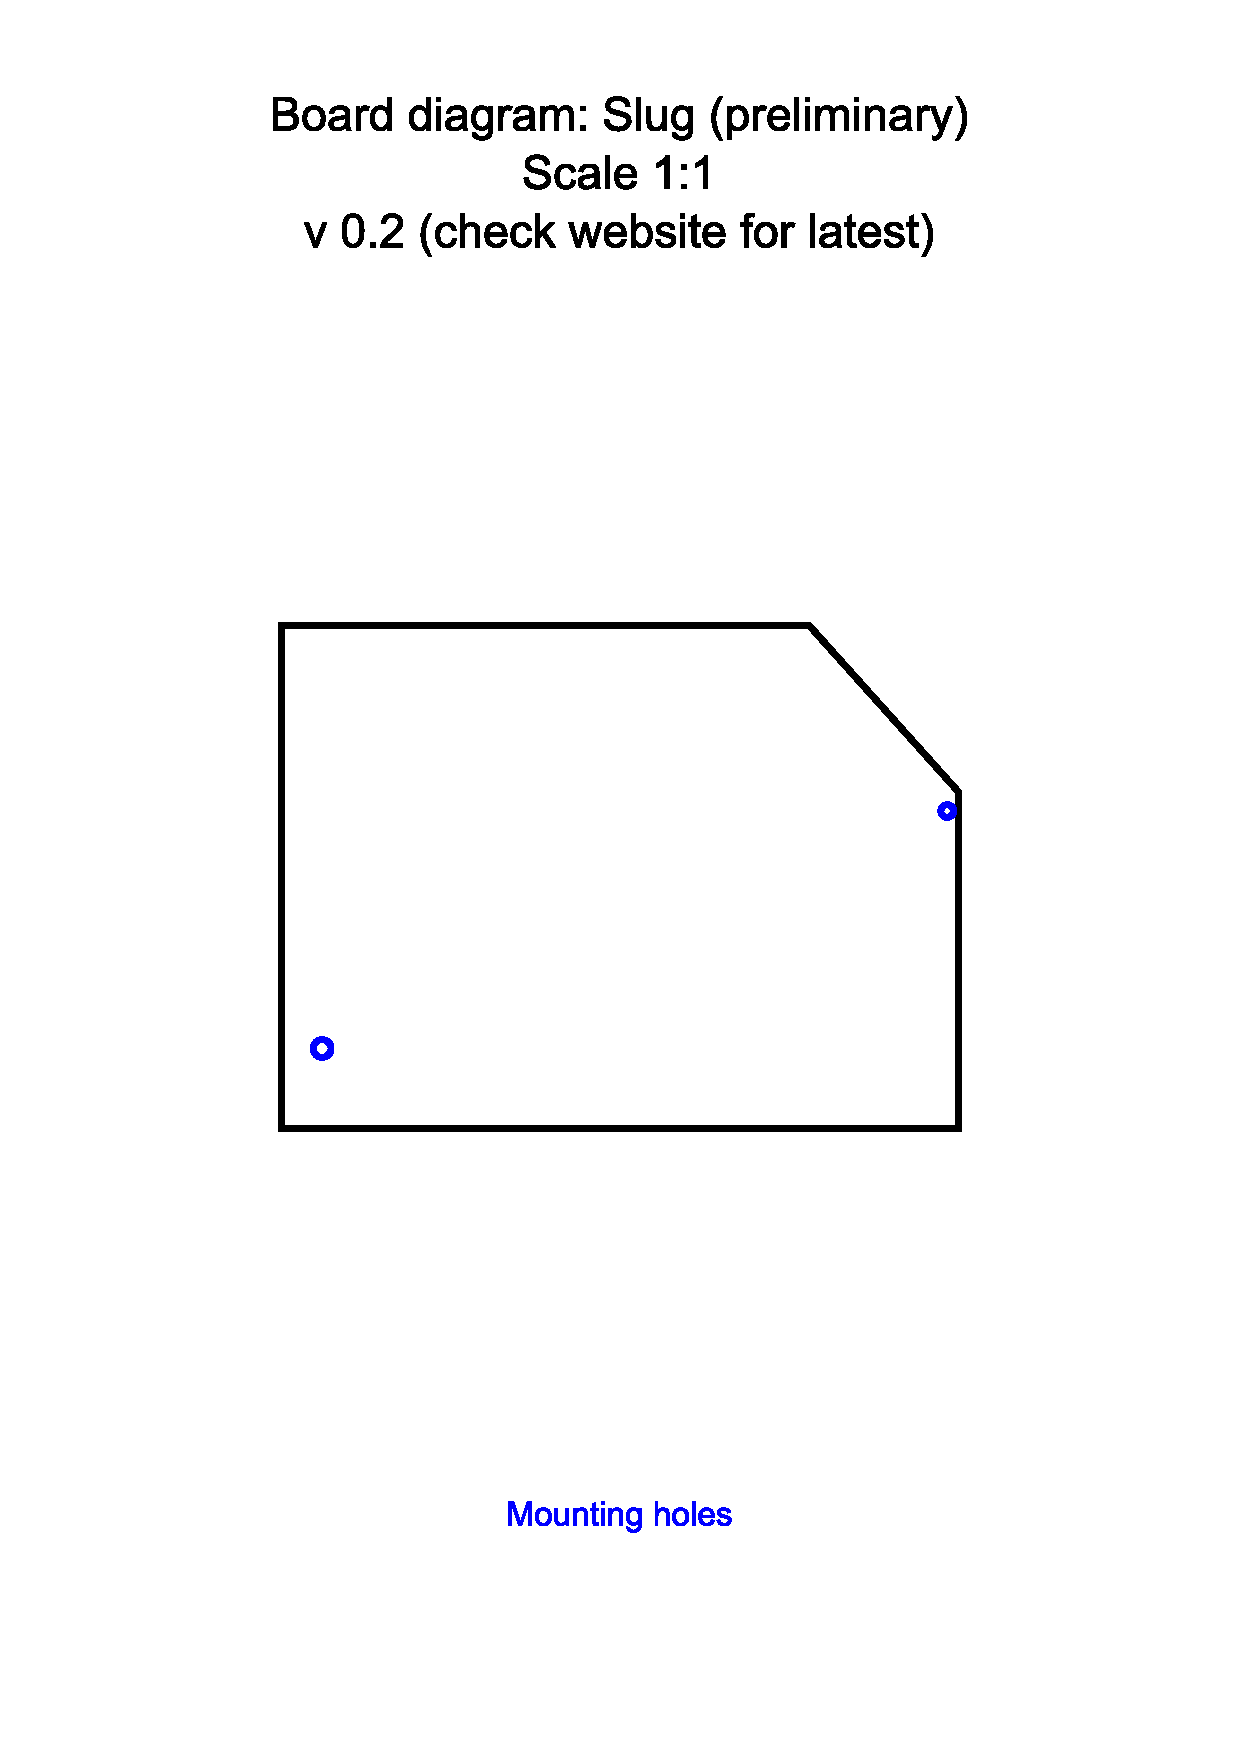
\includegraphics[width=4cm]{slug}  & Slug & 1 \\ \hline
\includegraphics[width=4cm]{battery}  & 12V Sealed Lead Acid battery & 1 \\ \hline
\includegraphics[width=4cm]{camcon}  & SR Connector & 4 \\ \hline
\includegraphics[width=4cm]{battery}  & 12V Sealed Lead Acid battery & 1 \\ \hline
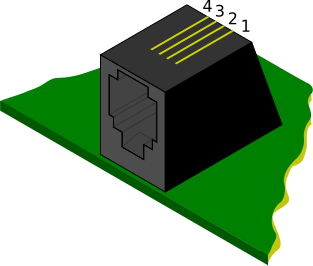
\includegraphics[width=4cm]{4p4c}  & RJ11 Cable & 5 \\ \hline
[photo]  & USB Memory Stick & 2 \\ \hline
[photo]  & Battery Charger & 1 \\ \hline
[photo]  & PCB Spacers & 16 \\ \hline
\end{longtable}

\end {document}
